\documentclass[11pt]{standalone}
\usepackage{amssymb}
\usepackage{amsmath}
\usepackage[no-math]{fontspec}
\usepackage{unicode-math}
\usepackage{libertinus}
\usepackage{pgf,xcolor}
\usepackage{tikz}
\usetikzlibrary{arrows.meta, backgrounds}
\usepackage{pgfplots}
\pgfplotsset{compat=newest}

\definecolor{my_darkgray}{HTML}{484949}
\definecolor{my_lightgray}{HTML}{F3F4F4}
\definecolor{my_darkblue}{HTML}{005A94}
\definecolor{my_lightblue}{HTML}{CCDEE9}
\definecolor{my_yellow}{HTML}{FFEC7F}
\definecolor{my_red}{HTML}{E60000}
\definecolor{my_orange}{HTML}{E87846}

% Koordinatensystem eines Teilbilds
\newcommand{\panelaxes}{%
    \draw[my_darkgray!25, thin] (-0.5, -0.5) grid (2.5, 2.5);
    \draw[-{Stealth[length=5pt]}, thick, my_darkgray] (-0.5, 0) -- (2.7, 0)
        node[right, font=\small] {$x$};
    \draw[-{Stealth[length=5pt]}, thick, my_darkgray] (0, -0.5) -- (0, 2.7)
        node[above, font=\small] {$y$};
    \node[below, font=\scriptsize, my_darkgray] at (1, 0) {$1$};
    \node[below, font=\scriptsize, my_darkgray] at (2, 0) {$2$};
    \node[left, font=\scriptsize, my_darkgray] at (0, 1) {$1$};
    \node[left, font=\scriptsize, my_darkgray] at (0, 2) {$2$};
    \draw[my_darkgray, dashed, thick] (0, 0) rectangle (1, 1);
}

\begin{document}
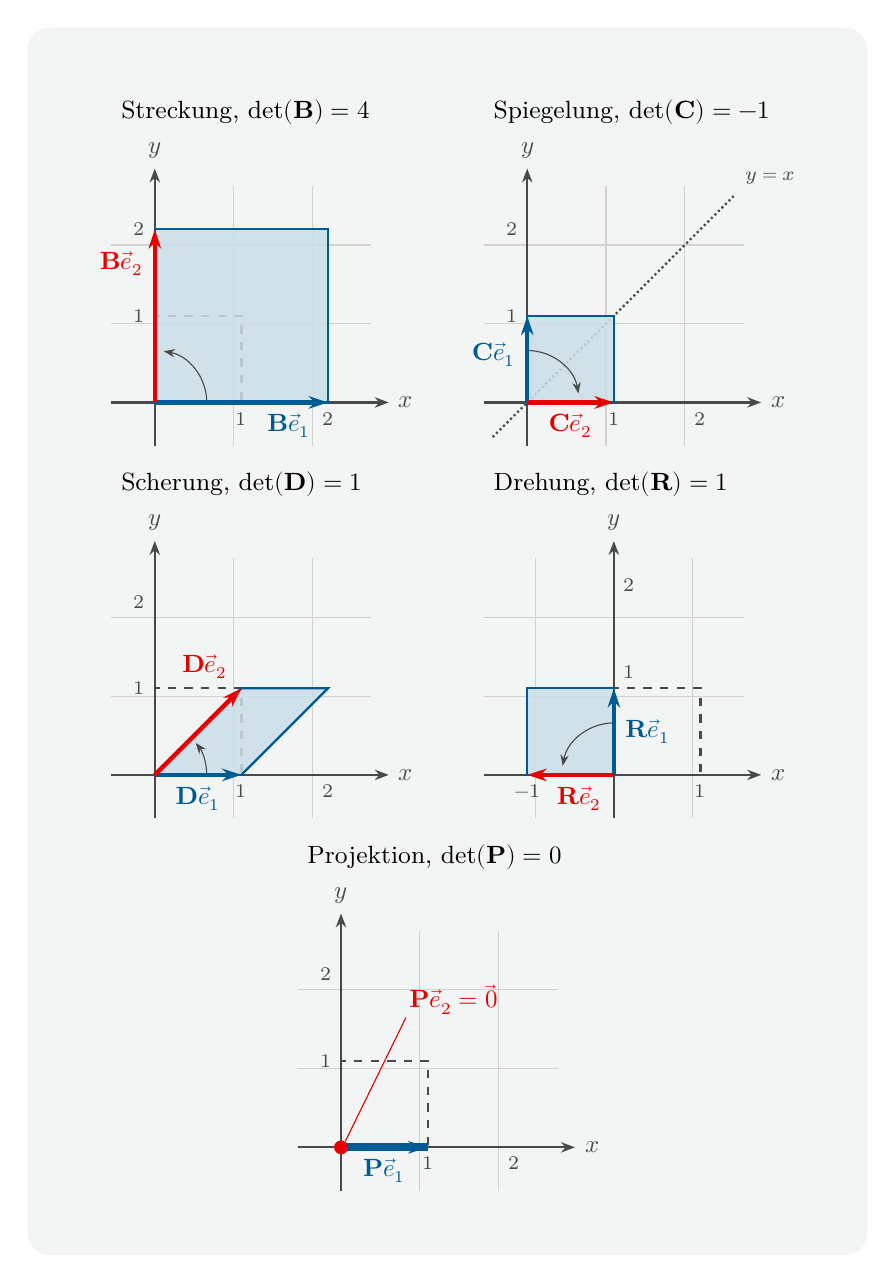
\begin{tikzpicture}[
    show background rectangle,
    background rectangle/.style={fill=my_lightgray, rounded corners=8pt},
    inner frame sep=0.8cm,
    x=1.1cm, y=1.1cm,
    vec/.style={-{Stealth[length=7pt, width=4.5pt]}, ultra thick},
    orient/.style={my_darkgray, -{Stealth[length=4pt]}}
]

% ---------------------------------------------------------------
%  Bild des Einheitsquadrats (gestrichelt) unter
%    B = (2 0; 0 2)  Streckung       C = (0 1; 1 0)  Spiegelung an y = x
%    D = (1 1; 0 1)  Scherung        R = (0 -1; 1 0) Drehung um 90 Grad
%    P = (1 0; 0 0)  Projektion auf x-Achse
%  Bild von e1 dunkelblau, Bild von e2 rot, Bogen = Orientierung
% ---------------------------------------------------------------

% ---- Streckung (oben links) ----
\begin{scope}[shift={(0, 8.6)}]
    \panelaxes
    \fill[my_lightblue, opacity=0.85] (0, 0) rectangle (2, 2);
    \draw[my_darkblue, thick] (0, 0) rectangle (2, 2);
    \draw[orient] (0:0.6) arc[start angle=0, end angle=80, radius=0.6];
    \draw[vec, my_darkblue] (0, 0) -- (2, 0);
    \draw[vec, my_red] (0, 0) -- (0, 2);
    \node[below, font=\small, my_darkblue] at (1.55, -0.02) {$\mathbf{B}\vec{e}_1$};
    \node[left, font=\small, my_red] at (-0.02, 1.6) {$\mathbf{B}\vec{e}_2$};
    \node[font=\small, anchor=west] at (-0.5, 3.35) {Streckung, $\det(\mathbf{B}) = 4$};
\end{scope}

% ---- Spiegelung (oben rechts) ----
\begin{scope}[shift={(4.3, 8.6)}]
    \panelaxes
    \draw[my_darkgray, densely dotted, thick] (-0.4, -0.4) -- (2.4, 2.4)
        node[above right, font=\scriptsize] {$y = x$};
    \fill[my_lightblue, opacity=0.85] (0, 0) rectangle (1, 1);
    \draw[my_darkblue, thick] (0, 0) rectangle (1, 1);
    \draw[orient] (90:0.6) arc[start angle=90, end angle=10, radius=0.6];
    \draw[vec, my_darkblue] (0, 0) -- (0, 1);
    \draw[vec, my_red] (0, 0) -- (1, 0);
    \node[left, font=\small, my_darkblue] at (-0.02, 0.55) {$\mathbf{C}\vec{e}_1$};
    \node[below, font=\small, my_red] at (0.5, -0.02) {$\mathbf{C}\vec{e}_2$};
    \node[font=\small, anchor=west] at (-0.5, 3.35) {Spiegelung, $\det(\mathbf{C}) = -1$};
\end{scope}

% ---- Scherung (Mitte links) ----
\begin{scope}[shift={(0, 4.3)}]
    \panelaxes
    \fill[my_lightblue, opacity=0.85] (0, 0) -- (1, 0) -- (2, 1) -- (1, 1) -- cycle;
    \draw[my_darkblue, thick] (0, 0) -- (1, 0) -- (2, 1) -- (1, 1) -- cycle;
    \draw[orient] (0:0.6) arc[start angle=0, end angle=38, radius=0.6];
    \draw[vec, my_darkblue] (0, 0) -- (1, 0);
    \draw[vec, my_red] (0, 0) -- (1, 1);
    \node[below, font=\small, my_darkblue] at (0.5, -0.02) {$\mathbf{D}\vec{e}_1$};
    \node[above left, font=\small, my_red] at (0.95, 1.0) {$\mathbf{D}\vec{e}_2$};
    \node[font=\small, anchor=west] at (-0.5, 3.35) {Scherung, $\det(\mathbf{D}) = 1$};
\end{scope}

% ---- Drehung (Mitte rechts) ----
% Das Bild liegt links der y-Achse, daher reicht dieses Teilbild von
% x = -1.5 bis 1.5 und ist um 1 nach rechts verschoben, damit es mit
% der Spiegelung darueber buendig ist.
\begin{scope}[shift={(5.3, 4.3)}]
    \draw[my_darkgray!25, thin] (-1.5, -0.5) grid (1.5, 2.5);
    \draw[-{Stealth[length=5pt]}, thick, my_darkgray] (-1.5, 0) -- (1.7, 0)
        node[right, font=\small] {$x$};
    \draw[-{Stealth[length=5pt]}, thick, my_darkgray] (0, -0.5) -- (0, 2.7)
        node[above, font=\small] {$y$};
    \node[below, font=\scriptsize, my_darkgray] at (-1, 0) {$-1$};
    \node[below, font=\scriptsize, my_darkgray] at (1, 0) {$1$};
    \node[above right, font=\scriptsize, my_darkgray] at (0, 1) {$1$};
    \node[above right, font=\scriptsize, my_darkgray] at (0, 2) {$2$};
    \draw[my_darkgray, dashed, thick] (0, 0) rectangle (1, 1);
    \fill[my_lightblue, opacity=0.85] (0, 0) rectangle (-1, 1);
    \draw[my_darkblue, thick] (0, 0) rectangle (-1, 1);
    \draw[orient] (90:0.6) arc[start angle=90, end angle=170, radius=0.6];
    \draw[vec, my_darkblue] (0, 0) -- (0, 1);
    \draw[vec, my_red] (0, 0) -- (-1, 0);
    \node[right, font=\small, my_darkblue] at (0.02, 0.5) {$\mathbf{R}\vec{e}_1$};
    \node[below, font=\small, my_red] at (-0.4, -0.02) {$\mathbf{R}\vec{e}_2$};
    \node[font=\small, anchor=west] at (-1.5, 3.35) {Drehung, $\det(\mathbf{R}) = 1$};
\end{scope}

% ---- Projektion (unten Mitte) ----
\begin{scope}[shift={(2.15, 0)}]
    \panelaxes
    \draw[my_darkblue, line width=3pt] (0, 0) -- (1, 0);
    \draw[vec, my_darkblue] (0, 0) -- (1, 0);
    \node[below, font=\small, my_darkblue] at (0.5, -0.02) {$\mathbf{P}\vec{e}_1$};
    \fill[my_red] (0, 0) circle (2.5pt);
    \draw[my_red, thin] (0.05, 0.07) -- (0.75, 1.5)
        node[above right, font=\small, inner sep=1pt] {$\mathbf{P}\vec{e}_2 = \vec{0}$};
    \node[font=\small, anchor=west] at (-0.5, 3.35) {Projektion, $\det(\mathbf{P}) = 0$};
\end{scope}

\end{tikzpicture}
\end{document}
